%% file: template.tex = LaTeX template for article-like report 
%% init: sometime 1993
%% last: Feb  8 2015  Rob Rutten  Deil
%% site: http://www.staff.science.uu.nl/~rutte101/rrweb/rjr-edu/manuals/student-report/

%% First read ``latex-bibtex-simple-manual.txt'' at
%% http://www.staff.science.uu.nl/~rutte101/Report_recipe.html

%% Start your report production by copying this file into your XXXX.tex.
%% Small changes to the header part will make it an A&A or ApJ manuscript.

%%%%%%%%%%%%%%%%%%%%%%%%%%%%%%%%%%%%%%%%%%%%%%%%%%%%%%%%%%%%%%%%%%%%%%%%%%%%
\documentclass{aa}   %% Astronomy & Astrophysics style class

\usepackage{graphicx,natbib,url,twoopt}
\usepackage[varg]{txfonts}           %% A&A font choice
\usepackage{hyperref}                %% for pdflatex
%%\usepackage[breaklinks]{hyperref}  %% for latex+dvips
%%\usepackage{breakurl}              %% for latex+dvips
\usepackage{pdfcomment}              %% for popup acronym meanings
\usepackage{acronym}                 %% for popup acronym meanings

\hypersetup{
  colorlinks=true,   %% links colored instead of frames
  urlcolor=blue,     %% external hyperlinks
  linkcolor=red,     %% internal latex links (eg Fig)
}

\bibpunct{(}{)}{;}{a}{}{,}    %% natbib cite format used by A&A and ApJ

\pagestyle{plain}   %% undo the fancy A&A pagestyle 

%% Add commands to add a note or link to a reference
\makeatletter
\newcommand{\bibnote}[2]{\@namedef{#1note}{#2}}
\newcommand{\biblink}[2]{\@namedef{#1link}{#2}}
\makeatother

%% Commands to make citations ADS clickers and to add such also to refs
%% May 2014: they give error stops ("Illegal parameter number ..."}
%%   for plain latex with TeX Live 2013; the ad-hoc fixes added below let
%%   latex continue instead of stop within these commands.
%%   Please let me know if you know a better fix!
%%   No such problem when using pdflatex.
\makeatletter
 \newcommandtwoopt{\citeads}[3][][]{%
   \nonstopmode%              %% fix to not stop at error message in latex
   \href{http://adsabs.harvard.edu/abs/#3}%
        {\def\hyper@linkstart##1##2{}%
         \let\hyper@linkend\@empty\citealp[#1][#2]{#3}}%   %% Rutten, 2000
   \biblink{#3}{\href{http://adsabs.harvard.edu/abs/#3}{ADS}}%
   \errorstopmode}            %% fix to resume stopping at error messages 
 \newcommandtwoopt{\citepads}[3][][]{%
   \nonstopmode%              %% fix to not stop at error message in latex
   \href{http://adsabs.harvard.edu/abs/#3}%
        {\def\hyper@linkstart##1##2{}%
         \let\hyper@linkend\@empty\citep[#1][#2]{#3}}%     %% (Rutten 2000)
   \biblink{#3}{\href{http://adsabs.harvard.edu/abs/#3}{ADS}}%
   \errorstopmode}            %% fix to resume stopping at error messages
 \newcommandtwoopt{\citetads}[3][][]{%
   \nonstopmode%              %% fix to not stop at error message in latex
   \href{http://adsabs.harvard.edu/abs/#3}%
        {\def\hyper@linkstart##1##2{}%
         \let\hyper@linkend\@empty\citet[#1][#2]{#3}}%     %% Rutten (2000)
   \biblink{#3}{\href{http://adsabs.harvard.edu/abs/#3}{ADS}}%
   \errorstopmode}            %% fix to resume stopping at error messages 
 \newcommandtwoopt{\citeyearads}[3][][]{%
   \nonstopmode%              %% fix to not stop at error message in latex
   \href{http://adsabs.harvard.edu/abs/#3}%
        {\def\hyper@linkstart##1##2{}%
         \let\hyper@linkend\@empty\citeyear[#1][#2]{#3}}%  %% 2000
   \biblink{#3}{\href{http://adsabs.harvard.edu/abs/#3}{ADS}}%
   \errorstopmode}            %% fix to resume stopping at error messages 
\makeatother

%% Acronyms
\newacro{ADS}{Astrophysics Data System}
\newacro{NLTE}{non-local thermodynamic equilibrium}
\newacro{NASA}{National Aeronautics and Space Administration}

%% Add popups with meaning to acronyms 
%% NB: only show up in Adobe Reader and do not work with \input or \include
\gdef\acp#1{%
  \pdfmarkupcomment[markup=Underline,color={1 1 1},author={{#1}},opacity=0]%
  {{#1}}{{\acl{#1}}}}

%% Spectral species
\def\MgI{\ion{Mg}{I}}          %% A&A; for aastex use \def\MgI{\ion{Mg}{1}} 
\def\MgII{\ion{Mg}{II}}        %% A&A; for aastex use \def\MgII{\ion{Mg}{2}} 

%% Hyphenation
\hyphenation{Schrij-ver}       %% Dutch ij is a single character

%%%%%%%%%%%%%%%%%%%%%%%%%%%%%%%%%%%%%%%%%%%%%%%%%%%%%%%%%%%%%%%%%%%%%%%%%%%%
\begin{document}  

%% simple header.  Change into A&A or ApJ commands for those journals

\twocolumn[{%
\vspace*{4ex}
\begin{center}
  {\Large \bf Stellar Spectra A. Basic Line Formation}\\[4ex]       
  {\large \bf Andreas Ellewsen$^{1}$}\\[4ex]
  \begin{minipage}[t]{15cm}
        $^1$ Institute of theoretical astrophysics\\

%  {\bf Abstract.} We learned how to write nice reports \ldots 

  \vspace*{2ex}
  \end{minipage}
\end{center}
}] 

%%%%%%%%%%%%%%%%%%%%%%%%%%%%%%%%%%%%%%%%%%%%%%%%%%%%%%%%%%%%%%%%%%%%%%%%%%%%
\section{Introduction}   \label{sec:Intro}
%%%%%%%%%%%%%%%%%%%%%%%%%%%%%%%%%%%%%%%%%%%%%%%%%%%%%%%%%%%%%%%%%%%%%%%%%%%%
This is the first of three numerical exercises in the course on Radiative processes in astrophysics (AST4310) at the University of Oslo. In this exercise we are to follow the steps of Annie Cannon, Cecilia Payne, and Marcel Minnaert. By doing this we hope to learn about the use of spectral lines in astophysics. 


%%%%%%%%%%%%%%%%%%%%%%%%%%%%%%%%%%%%%%%%%%%%%%%%%%%%%%%%%%%%%%%%%%%%%%%%%%%%
\section{Spectral Classification}    \label{sec:Specclas}
%%%%%%%%%%%%%%%%%%%%%%%%%%%%%%%%%%%%%%%%%%%%%%%%%%%%%%%%%%%%%%%%%%%%%%%%%%%%
The first part of this section deals with learning a little about how IDL functions.
You also make a fuction that adds all the numbers in an array together and gives you the result.
This function already exists in IDL, and is called TOTAL, but we make our own function anyway.
The function is called ADDUP, and looks exactly like the function written in the exercise text.
The function has been tested, and it passes all the test I've tried throwing at it (except of course those it will clearly fail, like strings). Note however that I will not be using IDL for this project since I know python better than IDL.

The second part of this section deals with LaTeX and gives instructions on how to write a good report.
Basically one is given a template and told a long list of things that are useful to know when writing reports, and then you use this knowledge for the rest of the exercise.

%%%%%%%%%%%%%%%%%%%%%%%%%%%%%%%%%%%%%%%%%%%%%%%%%%%%%%%%%%%%%%%%%%%%%%%%%%%%
\section{Saha-Boltzmann calibration of the Harvard sequence}   \label{sec:Saha}
%%%%%%%%%%%%%%%%%%%%%%%%%%%%%%%%%%%%%%%%%%%%%%%%%%%%%%%%%%%%%%%%%%%%%%%%%%%%
Here we want to explain the spectral-type sequence that was studied in the two first parts of the last section (which we ignored).
To start of we study figures 5 and 7 in the exercise text. 
Starting from the right of figure 5 one sees that the $H\beta$ line lies between $4762 \AA$ and $4954 \AA$. 
If one looks at figure 7 one sees that the only line between these two wavelengths is the Balmer $\beta$ line at $4861 \AA$. The Balmer $\beta$ line is the transition between $n = 4$ and $n = 2$. 
Considering that the spectrum we're looking at in figure 5 ranges between $3900 \AA$ and $5000 \AA$, which is in the visual part of the spectrum, the rest of the lines corresponding to hydrogen should all be in the Balmer series as well. 
This means that none of the lines share the same upper level, and that they all share the same lower level, namely $n = 2$.
This is the case for all of these named series. Sharing of the upper levels is a bit more complicated. 
If one looks at figure 7 one sees that Lyman $\alpha$ shares no upper level with anything. 
But Lyman $\beta$ shares the same upper level as Balmer $\alpha$. 
Figure 7 skips some of the transitions. 
But Lyman $\gamma$ shares upper level with Balmer $\beta$ and Paschen $\alpha$. 
It keeps going in this way for the rest of the transitions.

At this point Payne made the assumption that the strength of the absorption lines observed in stellar spectra scaled with the population density of the lower level of the corresponding transition. Assuming that most of the hydrogen is in the lower energy levels it is logical that most of the transitions must be going upwards in the levels, and thus they should scale with the population density of the lower levels. It turns out that this assumption assumption is not correct, but in general it is true that stellar absorption lines get stronger at larger lower-level population. We ignore this and continue with Payne's assumption anyway.

If we assume that the above is true. We can give som rough estimates of the strength ratios of the $\alpha$ lines in the HI Lyman, Balmer, Paschen and Brackett series. We see from figure 7 in the exercise that Lyman $\alpha$ releases about $10 eV$, while Balmer releases about $2 eV$, Paschen $0.5eV$ and Brackett about $0.25 eV$. Considering that our assumption means more transitions from lower levels, the Lyman $\alpha$ line should be much stronger than the Balmer. And the Balmer should be much stronger than the Paschen and so forth. 

Next we need to define some functions:

The Boltzmann distribution is defined
\begin{equation}
\frac{n_{r,s}}{N_r} = \frac{g_{r,s}}{U_r} e^{-\chi_{r,s}/kT} 
\end{equation}\label{Boltzmann}

The Partition function $U_r$ is defined as
\begin{equation}
 U_r = \sum_s g_{r,s} e^{-\chi_{r,s}/kT}
\end{equation}\label{Partition}

The Saha law reads
\begin{equation}
 \frac{N_{r+1}}{N_r} = \frac{1}{N_e}\frac{2U_{r+1}}{U_r}\bigg(\frac{2\pi m_e kT}{h^2}\bigg)^{3/2} e^{-\chi_r/kT}.
\end{equation}\label{Saha}

We will use this to study a fictional element known as Schadeenium(E).
Schadeenium has 
\begin{itemize}
\item
ionization energies $\chi_1 = 7$ eV for neutral E, $\chi_2 = 16$eV for E$^+$, $\chi_3 = 31$eV for E$^2+$, $\chi_4 = 51$eV for E$^3+$. 
\item
excitation energies that increase incrementally by $1$ eV: $\chi_{r,s} \equiv s -1$ eV in each stage
\item
statistical weights $g_{r,s} \equiv 1$ for all levels (r,s)
\end{itemize}

Table 1 on page 12 of the exercise shows different values of the 3 functions for our element.
When looking at this it is clear that the partition function is weakly dependent on temperature.
In the table with calulcations for the boltzmann function we see a steep decline in the population for higher levels.
The higher levels do fill up if one raises the temperature but the ground state always has the largest population.
From this it is clear that the lower levels are the most important ones. For real atoms the energy difference between levels 1 and 2 are usually larger than for E, and thus their partition functions are often well approixmated by the statistical weight of the ground state.

The reason for the difference in behaviour between the Saha and Boltzmann distributions is caused by the $(...)^{3/2}$ factor in front of the exponential in the Saha distribution. The Boltzmann distribution doesn't have this factor and thus it converges towards $g_{r,s}/U_r$ for hight T while Saha just keeps rising indefinitely.

Raising the temperature thus causes the distribution between the energy levels to spread out, and even if we don't get a lot of electrons in the higher energy levels, the thermal energy is high enough to cause ionization from the lower levels to the next ionization stage.

Thus we've found that when a gas is in thermal equilibrium we expect to find at most two ionization stages present. And for each ionization there is a steep decline in the population for each energy level.

With this in mind we compute the partition function $U_r$ for Schadeenium and print the values for levels $r =[0,3]$.
\begin{verbatim}
[ 1.10887478  1.10887488  1.10887488  1.10887488]
[ 1.45590319  1.45633511  1.45633513  1.45633513]
[ 2.23243073  2.27133987  2.27155094  2.27155097]
\end{verbatim}
Which is a perfect match to the values tabulated in the exercise text.

We then make a Boltzmann function in the program and check that it functions properly by printing the relative level population for $s = [0,10]$ for $T = 5000,10000,20000$. The output from the program is 
\begin{verbatim}
[  9.01815078e-01   8.85447148e-02   8.69376295e-03   8.53597128e-04
   8.38104353e-05   8.22892772e-06   8.07957280e-07   7.93292867e-08
   7.78894614e-09   7.64757688e-10   0.00000000e+00]
[  6.86858856e-01   2.15223692e-01   6.74392378e-02   2.11317385e-02
   6.62152166e-03   2.07481978e-03   6.50134114e-04   2.03716183e-04
   6.38334190e-05   2.00018738e-05   0.00000000e+00]
[ 0.44794223  0.25074559  0.1403604   0.07856984  0.04398121  0.02461946
  0.01378129  0.00771438  0.0043183   0.00241726  0.        ]
\end{verbatim}
which matches the values given in the exercise text.

The next step is to make a Saha function and test that for $r = [1,6]$ for $T = 20000$ and $e_{pressure} = 100$, and for $r = [1,6]$, with $T = 10000$ and $e_{pressure} = 100$. We print the results and get 
\begin{verbatim}
 2.72775113242e-10
0.000180278462885
0.632005363273
0.36781263824
1.71975186581e-06
----
0.000477757567228
0.94509484422
0.0544273981268
8.63969442555e-11
1.56819249959e-29
\end{verbatim}
Which matches the values given in the exercise, cofirming that the function works as it should.

THIS IS WHERE YOU SHOULD CONTINUE WRITING!!!!!!
THIS IS WHERE YOU SHOULD CONTINUE WRITING!!!!!!
THIS IS WHERE YOU SHOULD CONTINUE WRITING!!!!!!
THIS IS WHERE YOU SHOULD CONTINUE WRITING!!!!!!
THIS IS WHERE YOU SHOULD CONTINUE WRITING!!!!!!





\begin{itemize}
 \item 
 Note in the first table that the partition functions computed from (2) are of order unity and barely sensitive to temperature.
\item
In the second table, note the steep Boltzmann population decay with $\chi_{r,s}$ given by (1). It is less steep for higher temperature. The columns add up to unit y because the values in this table are scaled by $N_r$. They therefore depend on $U_r$, but the small variation between $U_1$ and $U_4$ in the first table produces a difference at two-digit significance only for $s = 1$ at $20 000 K$. The partition function $U_1$ of the neutral stage is the sum of only seven levels; the higher levels present in stages $r \ge 2$ contribute only marginally. The ground state always has the largest population.
\item
Inspect the third table, computed from (3). There are only two ionization stages significantly present per column. For T = 5000 K element E is predominantly neutral, for T = 10 000 K it is once ionized ($E^+$), for higher temperature stages $E^{2+}$ and $E^{3+}$ appear while $E$ and $E^+$ vanish.
\item
Explain from (1) and (3) why the Saha and Boltzmann distributions behave differently for increasing temperature.
\item
Speculate why ionization can fully deplete a stage even though excitation puts only a few atoms in levels below the ionization level. Hint: what parameter in the Saha distribution can cause equality between high-level and next-ion population at a given temperature?
\end{itemize}
\subsection{Saha-Boltzmann population of Shadeenium}
Now it is time to reproduce Shadee's tables. This is done by using python routines to compute $U_r$ from (2) and $n_{r,s}/N_r$ from (1), and $N_r/N$ from (3) for element E. All computations are done using cgs units.
%See Fig.~\ref{fig:XX}.
%%%%%%%%%%%%%%%%%%%%%%%%%%%%%%%%%%%%%%%%%%%%%%%%%%%%%%%%%%%%%%%%%%%%%%%%%%%%
\section{Fraunhofer line strengths and the curve of growth}   \label{sec:Fraunhofer}
%%%%%%%%%%%%%%%%%%%%%%%%%%%%%%%%%%%%%%%%%%%%%%%%%%%%%%%%%%%%%%%%%%%%%%%%%%%%


\subsection{Radiation through an isothermal layer}
It can be shown that the total emergent radiation from a layer with optical thickness $\tau(x)$ and temperature $T(x)$ is:
\begin{equation}\label{Radiation_general}
\begin{aligned}
 I_{\lambda} =& I_{\lambda}(0)e^{-\tau} + \int_0^\tau B_{\lambda}[T(x)]e^{-(\tau - \tau(x))}d\tau(x)
\end{aligned}
\end{equation}
If one assumes that the layer is isothermal, this implies that the optical thickness and temperature is independent of position inside the layer. Inserting this into equation \ref{Radiation_general} gives the following

\begin{equation*}
\begin{aligned}
I_{\lambda} =& I_{\lambda}(0)e^{-\tau} + \int_0^\tau B_{\lambda}[T(x)]e^{-(\tau - \tau(x)')}d\tau(x)'\\
	    =& I_{\lambda}(0)e^{-\tau} + B_{\lambda}(T)e^{-\tau}\int_0^\tau e^{\tau'}d\tau'\\
	    =& I_{\lambda}(0)e^{-\tau} + B_{\lambda}(T)e^{-\tau}(e^{\tau} - 1)\\
\end{aligned}
\end{equation*}

\begin{equation}\label{Radiation_isothermal}
 I_{\lambda} = I_{\lambda}(0)e^{-\tau} + B_{\lambda}(1 - e^{-\tau})
\end{equation}

\begin{figure}
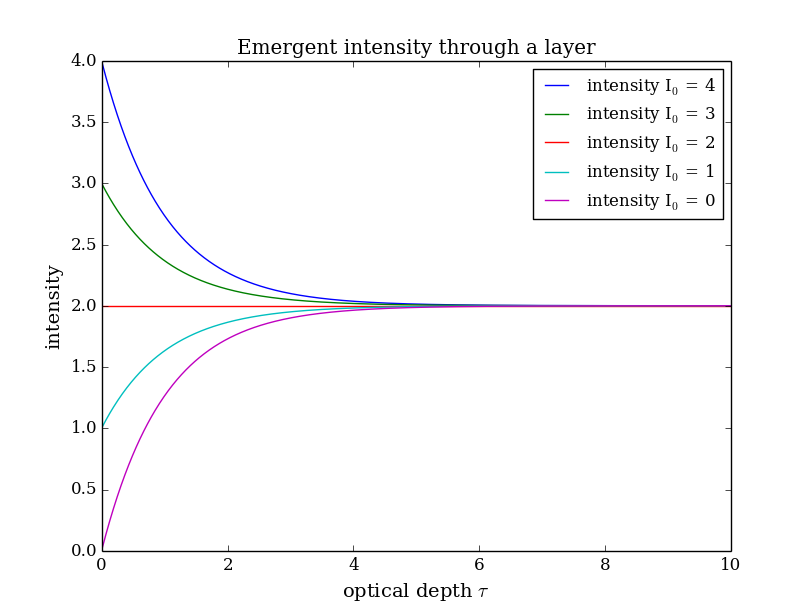
\includegraphics[width=.49\textwidth]{emergent_original.png}
\caption{As the optical depth increases, the intensity converges to the intensity of the Source function B.}
\label{emergent_original}
\end{figure}

\begin{figure}
 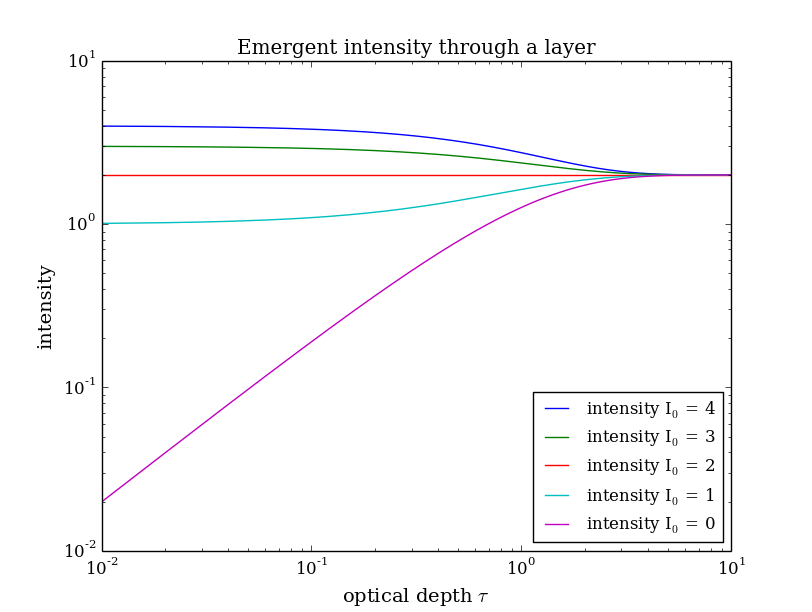
\includegraphics[width=.49\textwidth]{emergent_log.png}
 \caption{The emergent intensity with a logarthimic scale.}
 \label{emergent_log}
\end{figure}
Studying figures \ref{emergent_original} \& \ref{emergent_log} shows a few different things.
If one first considers cases where $\tau << 1$, the figures show that if $I_\lambda(0) = 0$, you get an exponential growth due to the source function B. And if $I_\lambda(0) > B_\lambda$ the intensity stays close to constant. This case corresponds to an ``optically thin'' medium. This is because whatever intensity that enters the medium passes straight through without being affected by the medium.

The opposite case where $\tau >> 1$ is called an ``optically'' thick medium, since all the incident radiation is absorbed before it is able to pass through, and is replaced by the radiation emitted by the medium itself. As seen in the plot, the emergent intensity becomes independent of optical depth for large $\tau$. Mathematically this can be seen by looking at equation \ref{Radiation_isothermal} and letting $\tau \rightarrow \infty$. In physical terms one can picture it such that both the incident radiation and the radiation emitted by the medium is absorbed while it is passing through the medium, but since the medium replenishes the radiation it is emitting along the path through it, this radiation is refilled as one goes through the medium.

From this it should be clear that optically thin mediums allow us to view radiation originating from the other side of the medium, while optically thick mediums absorb all of the incident radiation before it can pass through, thus blocking our view past them.

\subsection{Spectral lines from a solar reversing layer}
At this point we choose to use the Schuster-Schwarzschild model. Another name for this model is a reversing-layer model.
This model works on the assumption that the continous radiation, without spectral lines, is emitted by the surface of the star, and this radiation then irradiates a seperate layer around the star.
This layer is then hit by an intensity
\begin{equation}
 I_\lambda(0) = B_\lambda(T_{surface}).
\end{equation}\label{Surface layer}
This causes emission only at the wavelengths of spectral lines. 
Next, ones assumes that the star is optically thick, so that the surfrace radiates with the solution of equation \ref{Radiation_isothermal} where $\tau << 1$, meaning $I_\lambda = B_\lambda(T_{surface})$. This does not mean that shell has to be optically thick. The line-causing atoms in the shell have their own temperature $T_{layer}$, giving a local production of radiation in the layer for the line-wavelength $B_\lambda(T_{layer})\Delta\tau(x)$. Combining equation \ref{Radiation_isothermal} \& \ref{Reversing layer} yields
\begin{equation}
 I_\lambda =B_\lambda(T_{surface})e^{-\tau_\lambda} + B_\lambda(T_{layer})(1 - e^{-\tau_\lambda})
\end{equation}\label{Reversing layer}
Note that the opaqueness $\tau$ in equation \ref{Reversing layer} has gotten an index for wavelength, since it depends on wavelength.

\subsection{Voigt profile}
In reality spectral lines are not infinitely sharp delta functions. This can be attributed to Doppler shifts and Coloumb interactions between neighbouring particles. (Even if one could get rid of those effects, you would still have the uncertainty principle spreading it out a little.)

This broadening of the spectral line is described by the distribution
\begin{equation}
 \tau(u) = \tau(0)V(a,u)
\end{equation}\label{distribution}
where V is the Voigt function, and u describes the the wavelength separation from the center of the line such that
\begin{equation}
 u \equiv \Delta\lambda/\Delta\lambda_D
\end{equation}
where
\begin{equation}
 \Delta\lambda_D \equiv \frac{\lambda}{c} \sqrt{2kT/m}.
\end{equation}
Here m is the mass of the line-causing particles.
The a parameter measures the the Coloumb disturbances. For stellar atomspheres a is usually somewhere in the range $0.01 - 0.5$. The definition of the Voigt function is
\begin{equation}
 V(a,u) = \frac{1}{\Delta\lambda_D\sqrt{\pi}}\frac{a}{\pi}\int_{-\infty}^{+\infty}\frac{e^{-y^2}}{(u-y)^2 + a^2}dy
\end{equation}\label{Voigt}
The Voigt profile represents the convolution(smearing) of a Gauss profile using a Lorentz profile. Because of this it has a Gaussian shape close to line center, and Lorentzian wings on the edges.
This can be approximated by taking the sum instead of the convolution giving 
\begin{equation}
 V(a,u) = \frac{1}{\Delta\lambda_D\sqrt{\pi}} \bigg[e^{-u^2} + \frac{a}{\sqrt{\pi}u^2}\bigg]
\end{equation}\label{Voigt_approx}

For those using IDL to do calculations, the voigt function is ready for use through the appropriately named function voigt.
Since I use python we instead have to use the fact that the voigt function can be written
\begin{equation}
 V(x;\sigma,\gamma) = \frac{Re[w(z)]}{\sigma \sqrt{2\pi}}
\end{equation}
where Re[w(z)] is the real part of the Faddeeva function evaluated for 
\[
 z = \frac{x + i\gamma}{\sqrt{2}\sigma} ~,~ a = \frac{\sigma}{\sqrt{2}\sigma} ~,~ u = \frac{x}{\sqrt{2}\sigma}.
\]
In this case the factor $\Delta\lambda_D = \sqrt{2}\sigma$.
Luckily for us the Faddeeva function can be found in the special module of the scipy package for python, so that is what we will be using. If we plot this function for different values of $a$ for $u = [-10, 10]$ we get figure \ref{voigt_orig}.
\begin{figure}
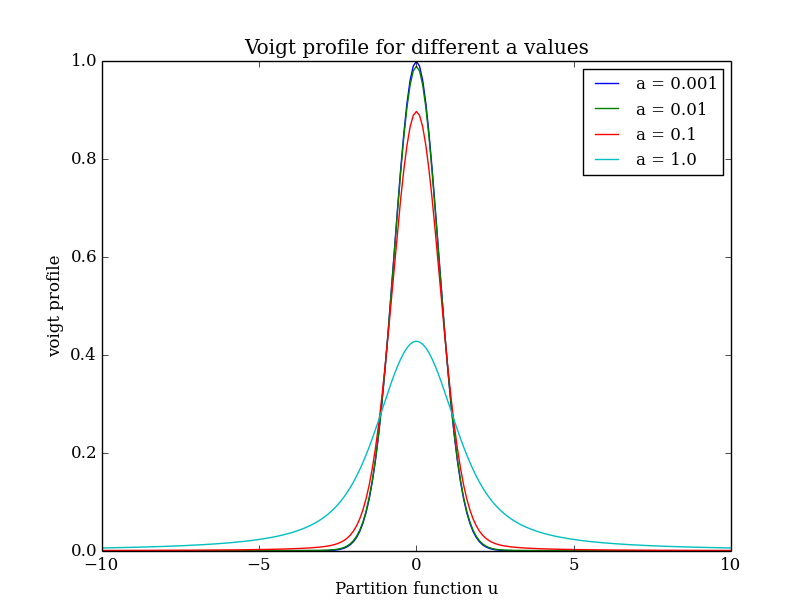
\includegraphics[width=.49\textwidth]{voigt_original.png}
\caption{Voigt profile for different values of a.}
\label{voigt_orig}
\end{figure}
To study this we plot the same, but this time with a logarthimic scale for the y axis. The plot can be seen in figure \ref{voigt_ylog}.
\begin{figure}
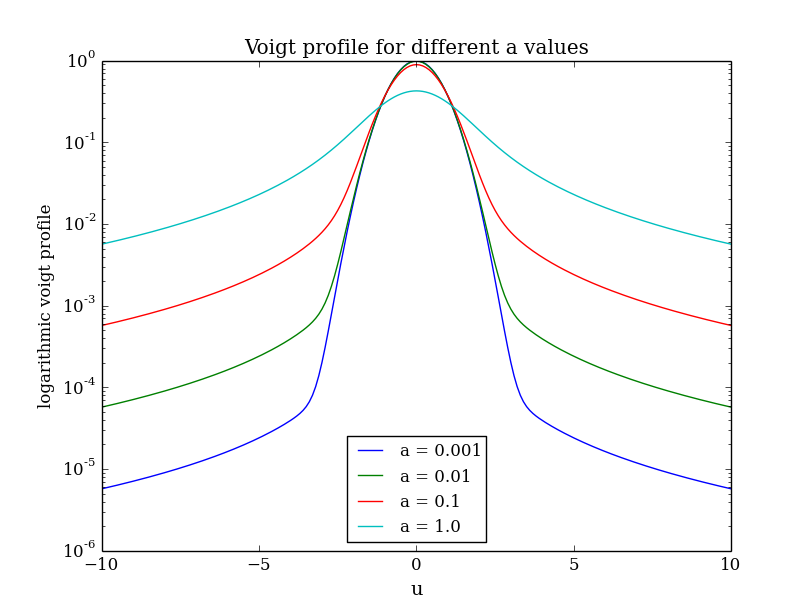
\includegraphics[width=.49\textwidth]{voigt_ylog.png}
\caption{Logarithmic voigt profile for different values of a.}
\label{voigt_ylog}
\end{figure}
Using approximation \ref{Voigt_approx} it is clear that the the exponential term vanishes very quickly as $|u|$ increases, leaving us with
\[
 V(a,u) \approx \frac{a}{\Delta\lambda_D\pi u^2} 
\]
which gives the functions the same form on the wings just scaled by the factor $a$.

\subsection{Emergent line profiles}
We now have both functions for intensity and for the distribution of the optical depth. If we now combine equation \ref{Radiation_isothermal} \& \ref{distribution} we should be able to compute and plot stellar spectral line profiles!
To do this we use values that fit well with the solar photosphere and plot what it looks like in the visible spectrum.
The values we will be using are $T_{surface} = 5700 K$, $T_{layer} = 4200 K$, $a = 0.01$, $\lambda = 5000 \AA$.
We start by plotting the intensity against $u$ for $\tau(0) = 1$. This results in figure \ref{emergent_line_orig_5000}.
\begin{figure}
 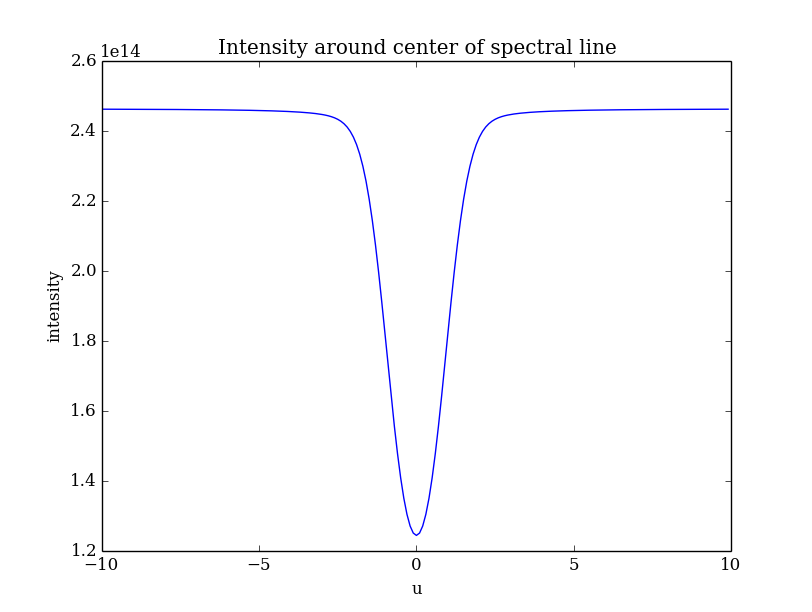
\includegraphics[width=.49\textwidth]{emergent_line_orig_5000.png}
 \caption{Spectral lines for wavelength $5000 ~\AA$.}
 \label{emergent_line_orig_5000}
\end{figure}

\begin{itemize}
 \item 
 Explain profile shapes for $\tau(0) << 1$.
 \item 
 Why is there a low-intensity saturation limit for $\tau >> 1$?
 \item 
 Why do the line wings develop only for very large $\tau(0)$?
 \item 
 Where do the wings end?
 \item 
 For which values of $\tau(0)$ is the layer optically thin,respectively optically thick, at line center?
 And at $u = 5$ ?
 \item
 Now study the dependence of these line profiles on wavelength by repeating the above for $\lambda = 2000 \AA$ (ultraviolet) and $\lambda = 10000 \AA$ (near infrared). What sets the top value $I_{cont}$ and the limit value reached at line center 	by $I(0)$? Check these values by computing them directly on the command line. What happens to these values at other wavelengths?
\end{itemize}

Next we study the behaviour of the line for $\tau(0)$ in the range $\log \tau(0) = [-2, 2]$.
This results in figure \ref{emergent_line_log_2000}.
\begin{figure}
 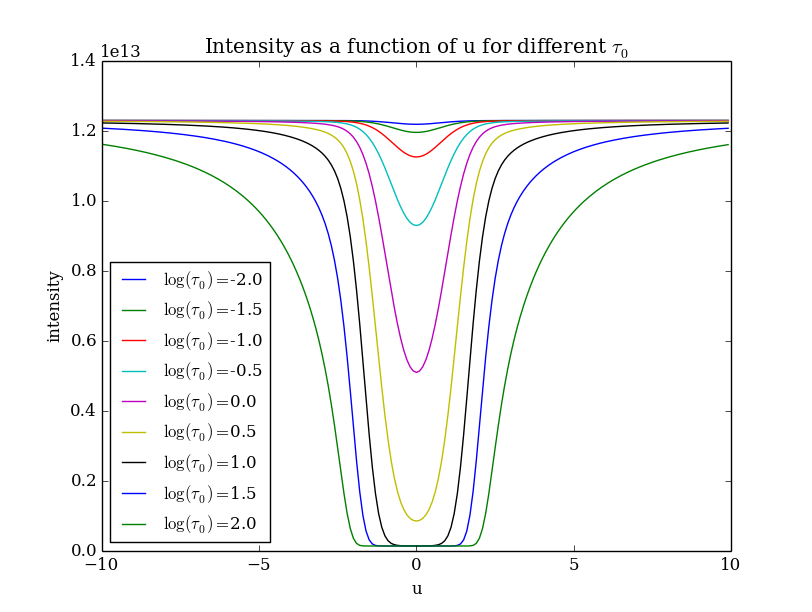
\includegraphics[width=.49\textwidth]{emergent_line_log_2000.png}
 \caption{Spectral lines for different choices of $\tau(0)$.}
 \label{emergent_line_log_2000} 
\end{figure}
Looking at the spectral lines for different wavelengths reveal a difference in intensity. This can be seen in figure \ref{emergent_line_orig}.

To check the behaviour for different wavelengths we plot the results for $\lambda = 5000$ \& $10000$ in figures  \ref{emergent_line_log_5000} $\&$ \ref{emergent_line_log_10000}.

\begin{figure}
 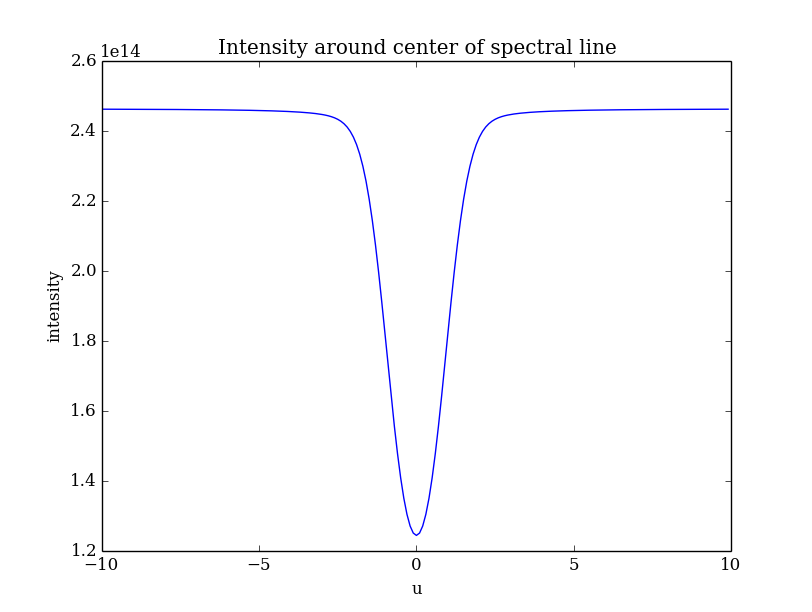
\includegraphics[width=.49\textwidth]{emergent_line_orig.png}
 \caption{Spectral lines for different wavelengths.}
 \label{emergent_line_orig}
\end{figure}
\begin{figure}
 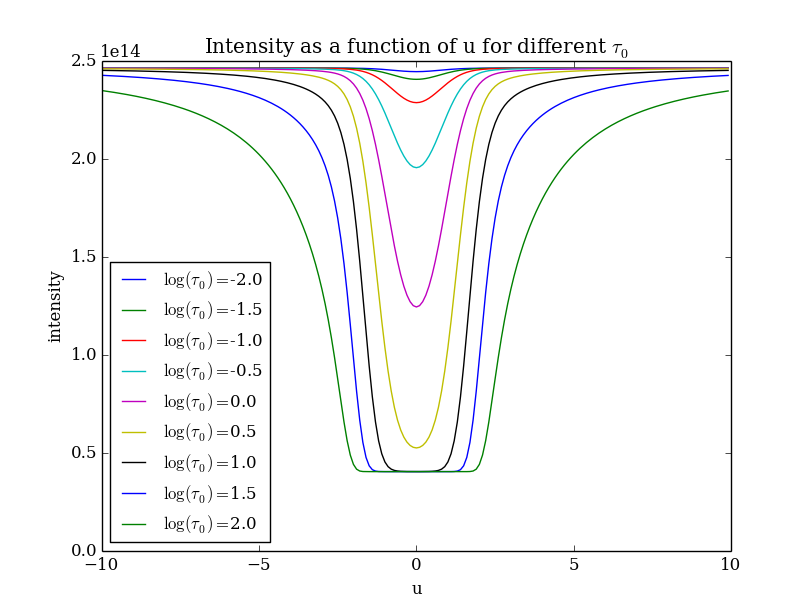
\includegraphics[width=.49\textwidth]{emergent_line_log_5000.png}
 \caption{Spectral lines for different choices of $\tau(0)$.}
 \label{emergent_line_log_5000} 
\end{figure}
\begin{figure}
 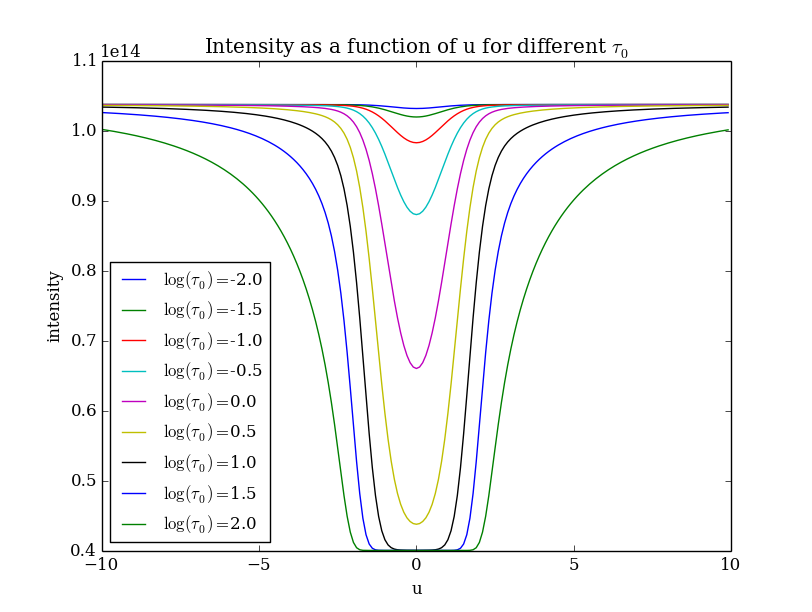
\includegraphics[width=.49\textwidth]{emergent_line_log_10000.png}
 \caption{Spectral lines for different choices of $\tau(0)$.}
 \label{emergent_line_log_10000} 
\end{figure}

\begin{itemize}
 \item 
 Explain profile shapes for $\tau(0) << 1$.
 \item 
 Why is there a low-intensity saturation limit for $\tau >> 1$?
 \item 
 Why do the line wings develop only for very large $\tau(0)$?
 \item 
 Where do the wings end?
 \item 
 For which values of $\tau(0)$ is the layer optically thin,respectively optically thick, at line center?
 And at $u = 5$ ?
 \item
 Now study the dependence of these line profiles on wavelength by repeating the above for $\lambda = 2000 \AA$ (ultraviolet) and $\lambda = 10000 \AA$ (near infrared). What sets the top value $I_{cont}$ and the limit value reached at line center 	by $I(0)$? Chek these values by computing them directly on the command line. What happens to these values at other wavelengths?
\end{itemize}

Since some observed spectra are measured without absolute intensity calibration it useful to scale the spectrum to the local continuum intensity by plotting $I_\lambda/I_{cont}$. Plotting this for the same 3 wavelengths reults in figure \ref{emergent_line_scaled_different}.
\begin{figure}[hbtp]
 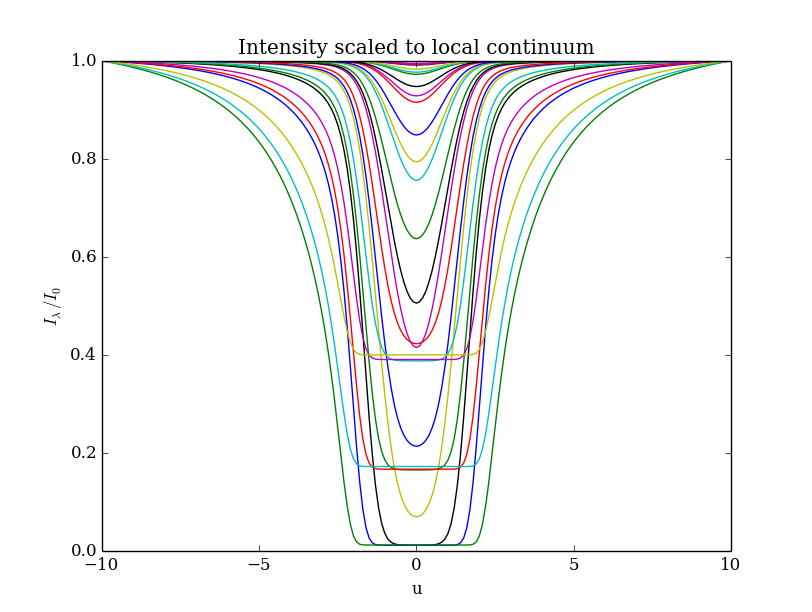
\includegraphics[width=.49\textwidth]{emergent_line_scaled_different.png}
 \caption{Spectral lines for different choices of $\tau(0)$.}
 \label{emergent_line_scaled_different} 
\end{figure}

\subsection{The equivalent width of spectral lines}
From the profile plots one can see that the growth of the absorption feature for increasing $\tau(0)$is faster for small $\tau(0)$ than for larger $\tau(0)$. Because of this, Minnaert and his coworkers introduced the equivalent width $W_\lambda$ as a line-strength parameter to measure this effect. It measures the integrated line depression in the normalized spectrum
\begin{equation}
 W_\lambda = \int \frac{I_{cont}-I(\lambda)}{I_{cont}}d\lambda.
\end{equation}\label{eqw}
To test this effectively we make a profile function that returns a Schuster-Schwarzschild profile, given $a$, $\tau$, and $u$.  Setting $a = 0.1$, $\tau(0) = 100$ and plotting this for $ u = [-200,200]$ returns figure \ref{eqw_ss}.
\begin{figure}[hbtp]
 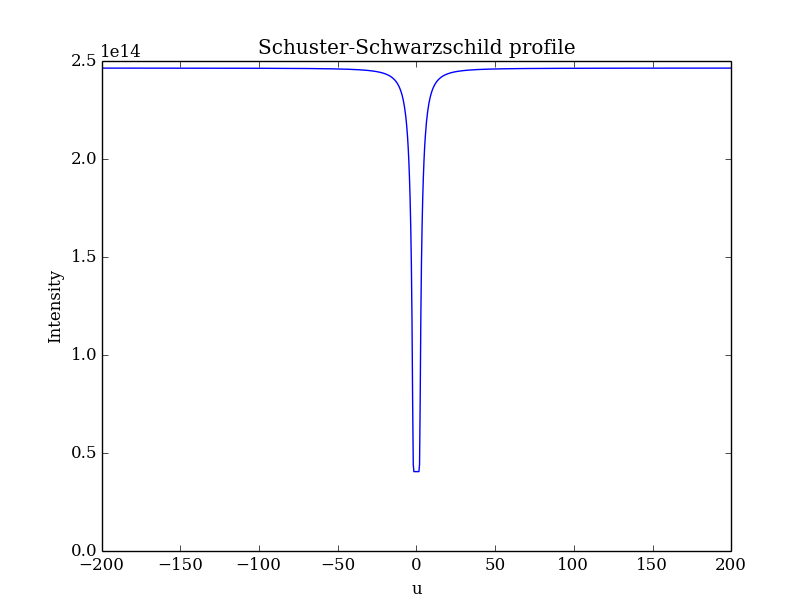
\includegraphics[width=.49\textwidth]{eqw_ss.png}
 \caption{Schuster-Schwarzschild profile.}
 \label{eqw_ss} 
\end{figure}

Next we compute the line depth in relative units(the integrand in equation \ref{eqw}. Plotting this versus u gives figure \ref{eqw_rel}.
\begin{figure}[hbtp]
 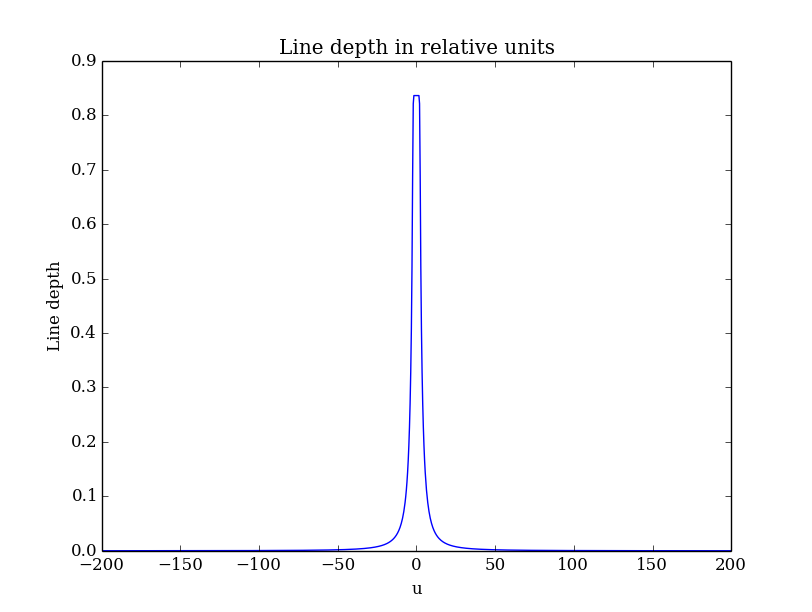
\includegraphics[width=.49\textwidth]{eqw_rel.png}
 \caption{Line depth in relative units.}
 \label{eqw_rel} 
\end{figure}

In this test case we get an equivalent width $W_\lambda = 7.5$.

\subsection{The curve of growth}
The point of the equivalent width was that it could be used to measure the number of atoms in the reversing layer. This should set the opaqueness $\tau(0)$ of the layer. The profile plots show that the profile growth is only linear with $\tau(0)$ for $\tau(0) <<1$. The curve of growth shows the full dependence; the growth of the line strength with the line-causing density.

To study this we plot $\log W_\lambda$ against $\log \tau(0)$ in figure \ref{growth}.

\begin{figure}[hbtp]
 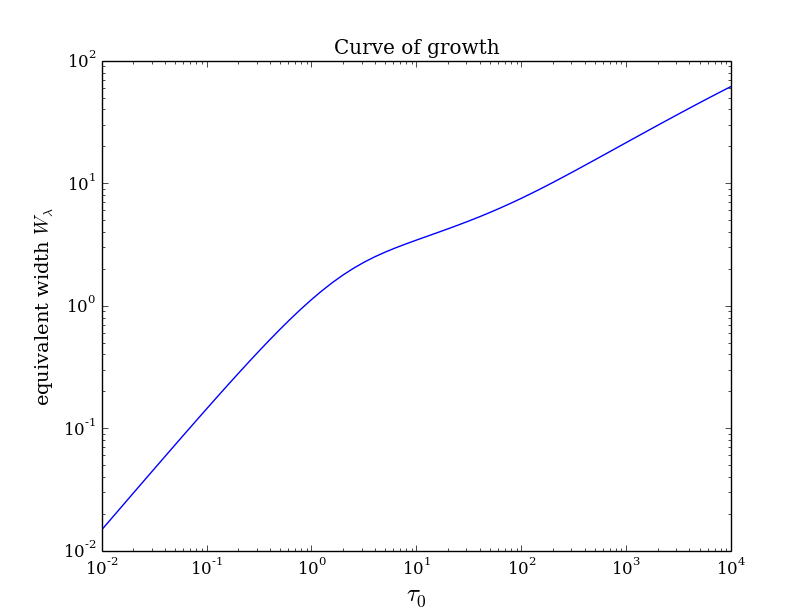
\includegraphics[width=.49\textwidth]{growth.png}
 \caption{Curve of Growth.}
 \label{growth} 
\end{figure}
\begin{itemize}
 \item 
 Explain what happens in the three different parts
 \item 
 The first part has slope 1:1 ,the third has slope 1:2 in this log-log plot. Why?
 \item 
 Which parameter controls the location of the onset of the third part? Give a rough estimate of its value for solar ironlines through comparison with figure 14 in the assignment.
 \item 
 Final: of which parameter should you raise the numerical value in order to produce emission lines instead of absorption lines? Change it accordingly and rerun your programs to produce emission profiles and an emission-line curve of growth. Avoid plotting negative $W_\lambda$ values logarithimically by plotting the absoulte value of equivalent width.
\end{itemize}

%%%%%%%%%%%%%%%%%%%%%%%%%%%%%%%%%%%%%%%%%%%%%%%%%%%%%%%%%%%%%%%%%%%%%%%%%%%%
\section{Conclusions} \label{sec:conclusions}
%%%%%%%%%%%%%%%%%%%%%%%%%%%%%%%%%%%%%%%%%%%%%%%%%%%%%%%%%%%%%%%%%%%%%%%%%%%%
insert conclusions
%%%%%%%%%%%%%%%%%%%%%%%%%%%%%%%%%%%%%%%%%%%%%%%%%%%%%%%%%%%%%%%%%%%%%%%%%%%%
\begin{acknowledgements}
\end{acknowledgements}

%%%%%%%%%%%%%%%%%%%%%%%%%%%%%%%%%%%%%%%%%%%%%%%%%%%%%%%%%%%%%%%%%%%%%%%%%%%%
%% references
\bibliographystyle{aa-note} %% aa.bst but adding links and notes to references
%%\raggedright              %% only for adsaa with dvips, not for pdflatex
%\bibliography{XXX}          %% XXX.bib = your Bibtex entries copied from ADS

\end{document}


